\section{Camada de Redes}

    \subsection{Introdução}

        \begin{itemize}[left=0.5cm, align=left, nosep]
            \item \textbf{Função principal:} fornece o transporte de segmentos dos hospedeiros de origem até os hospedeiros de destino. \\        
                $\hookrightarrow$ \textbf{Transmissor:} encapsula os segmentos em datagramas e encaminha para a camada de enlace; \\
                $\hookrightarrow$ \textbf{Receptor:} entrega os segmentos ao protocolo da camada de transporte.
        \end{itemize}

        \begin{center}
            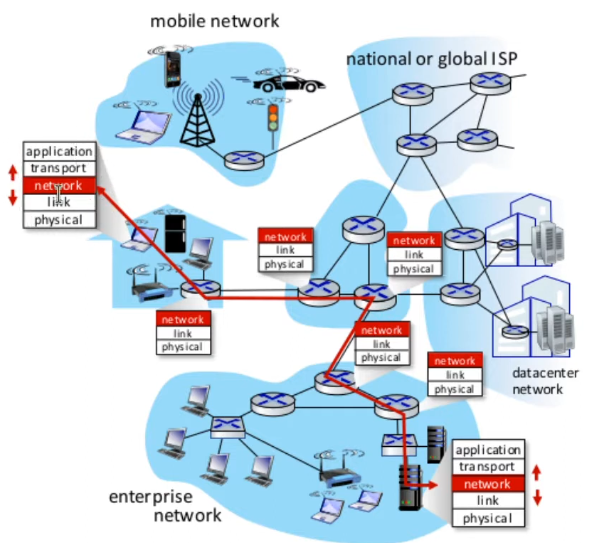
\includegraphics[width=0.65\textwidth]{img/cap-04/camada-de-redes-introd.png}
        \end{center}

        \begin{itemize}[left=0.5cm, align=left, nosep]
            \item A camada de redes deve estar implementada em todos os dispositivos ao longo da rota entre origem e destino.
        \end{itemize}

        \subsubsection*{Roteadores}
            \begin{itemize}[left=0.5cm, align=left, nosep]
            \item \textbf{Função :} \\
                $\hookrightarrow$ Examinar os cabeçalhos dos datagramas IP para extrair o endereço de destino; \\
                $\hookrightarrow$ Decidir para qual interface de saída o pacote será encaminhado.
            \end{itemize}

        \subsubsection*{Funções Principais da Camada de Rede}
            \begin{itemize}[left=0.5cm, align=left, nosep]
                \item \textbf{Encaminhamento:} move pacotes de uma interface de entrada para a interface de saída apropriada;
                \item \textbf{Roteamento:} determina a rota da origem até o destino (definida por algoritmos de roteamento).
            \end{itemize}

            \textbf{Analogia:} Fazer uma viagem
            \begin{itemize}[left=0.5cm, align=left, nosep]
                \item \textbf{Encaminhamento:} decisão tomada em cada encruzilhada;
                \item \textbf{Roteamento:} processo de definir todo o caminho de origem até o destino.
            \end{itemize}

            \begin{center}
                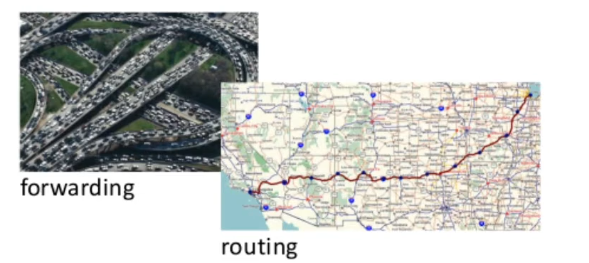
\includegraphics[width=0.55\textwidth]{img/cap-04/viagem.png}
            \end{center}

        \subsubsection*{Plano de Dados}
            \begin{itemize}[left=0.5cm, align=left, nosep]
                \item Local por dispositivo, função implementada por roteador;
                \item Ao receber um datagrama, o roteador analisa o cabeçalho e decide o encaminhamento.
            \end{itemize}

            \begin{center}
                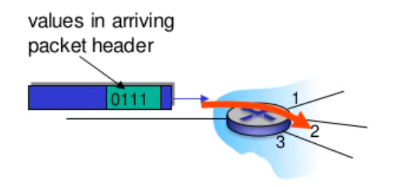
\includegraphics[width=0.65\textwidth]{img/cap-04/plano-de-dados.png}
            \end{center}

        \subsubsection*{Plano de Controle}
            \begin{itemize}[left=0.5cm, align=left, nosep]
                \item Lógica de toda a rede, determinando como datagramas são roteados de origem até destino;
                \item Implementações possíveis:
                
                \begin{enumerate}[left=0.5cm, align=left, nosep]
                    
                    \item \textbf{Algoritmos tradicionais de roteamento :} \\
                        $\hookrightarrow$ Implementados nos roteadores; \\
                        $\hookrightarrow$ Cada roteador executa uma parte do algoritmo de forma distribuída.
                    
                    \begin{center}
                        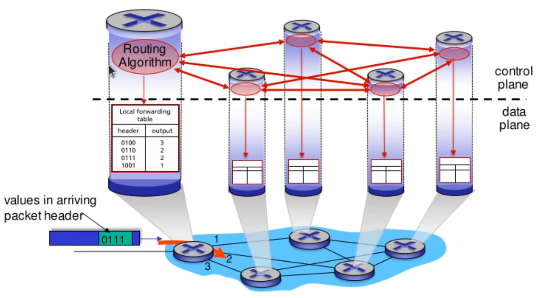
\includegraphics[width=0.6\textwidth]{img/cap-04/algorimo-roteamento.png}
                    \end{center}
                    
                    \item \textbf{SDN (Software Defined Networking) :} \\
                        $\hookrightarrow$ Implementado em controladores remotos; \\
                        $\hookrightarrow$ Controladores calculam e instalam as tabelas de encaminhamento nos roteadores.
                    
                    \begin{center}
                        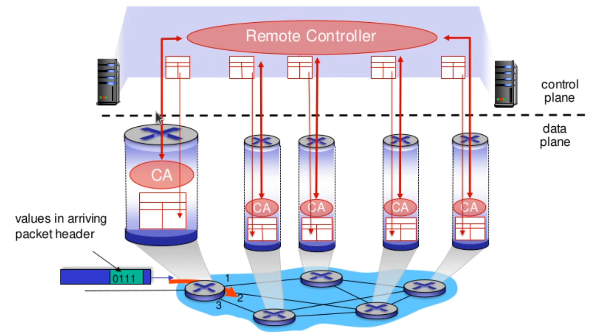
\includegraphics[width=0.6\textwidth]{img/cap-04/sdn.png}
                    \end{center}
                
                \end{enumerate}

            \end{itemize}

        \subsubsection*{Modelo de Serviço de Redes para Datagramas}
            \begin{itemize}[left=0.5cm, align=left, nosep]
                \item \textbf{Serviços para datagramas individuais :} \\
                    $\hookrightarrow$ Garantia de entrega; \\
                    $\hookrightarrow$ Garantia de entrega com atraso menor que 40 ms; \\
                    $\hookrightarrow$ Garantia de integridade; \\
                    $\hookrightarrow$ Garantia de confiabilidade.
                \item \textbf{Serviços para fluxos de datagramas :}
                    $\hookrightarrow$ Entrega em ordem; \\
                    $\hookrightarrow$ Garantia de taxa mínima de transferência; \\
                    $\hookrightarrow$ Restrição de variação de atraso (jitter).
            \end{itemize}

        \textbf{Modelo da Internet:} \textit{"Best Effort"} — não há garantias de entrega, temporização, ordenação ou taxa mínima de transmissão.

        \begin{table}[h!]
            \centering
            \renewcommand{\arraystretch}{1.3}
            \setlength{\tabcolsep}{3pt}
            \arrayrulecolor{blue}
            \begin{tabular}{|c|c|cccc|}
                \hline
                \textbf{Network Architecture} & \textbf{Service Model} &
                \multicolumn{4}{c|}{\textbf{Quality of Service (QoS) Guarantees?}} \\ \cline{3-6}
                & & \textbf{Bandwidth} & \textbf{Loss} & \textbf{Order} & \textbf{Timing} \\ \hline
                Internet & best effort & none & no & no & no \\ \hline
                ATM & Constant Bit Rate & Constant rate & yes & yes & yes \\ \hline
                ATM & Available Bit Rate & Guaranteed min & no & yes & no \\ \hline
                Internet & Intserv (RFC 1633) & yes & yes & yes & yes \\ \hline
                Internet & Diffserv (RFC 2475) & possible & possibly & possibly & no \\ \hline
            \end{tabular}
            \caption{Comparação de garantias de QoS entre diferentes arquiteturas e modelos de serviço.}
        \end{table}

        \subsubsection*{Reflexões sobre o Serviço “Best Effort”}
            \begin{itemize}[left=0.5cm, align=left, nosep]
                \item A simplicidade do mecanismo permitiu o crescimento da Internet;
                \item Na prática, há \textbf{superprovisionamento} de recursos para evitar congestionamentos;
                \item Há múltiplos mecanismos de \textbf{replicação e distribuição de conteúdo}, mantendo dados próximos dos usuários;
                \item Muitos serviços replicam conteúdo localmente, inclusive no provedor de acesso;
                \item O controle de congestionamento é eficiente em \textbf{serviços elásticos} — aplicações que usam toda a banda disponível.
            \end{itemize}

    \subsection{O tem dentro de um roteador ?}
        
        \begin{itemize}[left=0.5cm, align=left, nosep]
            \item \textbf{Arquitetura geral de um roteador :}
        
            \begin{center}
                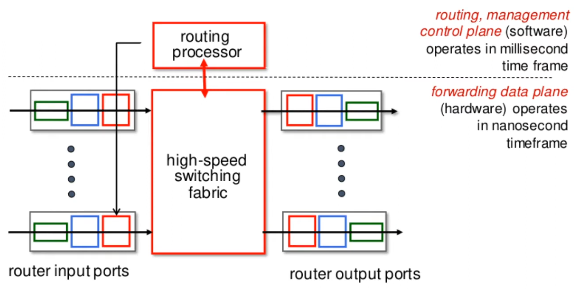
\includegraphics[width=0.65\textwidth]{img/cap-04/arquitetura-geral-roteador.png}
            \end{center}

            \item \textbf{Porta de Entrada :}
            
            \begin{center}
                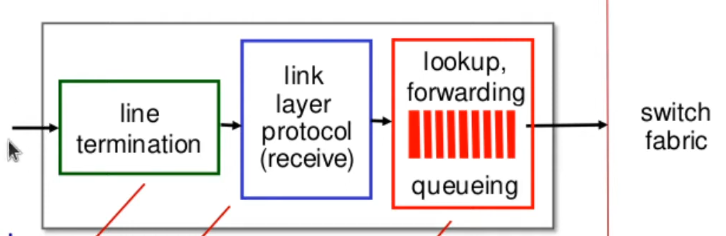
\includegraphics[width=0.55\textwidth]{img/cap-04/porta-de-entrada.png}
            \end{center}
            
            \item \textbf{Caixa Verde (Camada Física):} recepção dos bits;
            \item \textbf{Azul (Camada de Enlace):} Ethernet;
            \item \textbf{Vermelho:} operações de checagem do endereço de destino do pacote (lookup); \\
                $\hookrightarrow$ Objetivo da interface: encaminhar o pacote para a matriz de comutação na velocidade de linha; \\
                $\hookrightarrow$ Enfileiramento dos pacotes para evitar perdas em caso de chegada de datagramas for superior à capacidade \\
                $\hookrightarrow$ Decisão de encaminhamento :
                \begin{itemize}
                    \item Tradicional: Encaminhamento é baseado somente no endereço de IP do destino contido no cabeçalho;
                    \item Generalizado: Encaminhamento é baseado em qualquer informação contida no cabeçalho do datagrama
                \end{itemize}
            
        \end{itemize}

        \subsubsection*{Decisão de Encaminhamento :} 
    
            \begin{itemize}[left=0.5cm, align=left, nosep]
                \item O roteador possui uma tabela de encaminhamento que referencia endereços de destino e indica a interface de saída correspondente.
            
                \begin{center}
                    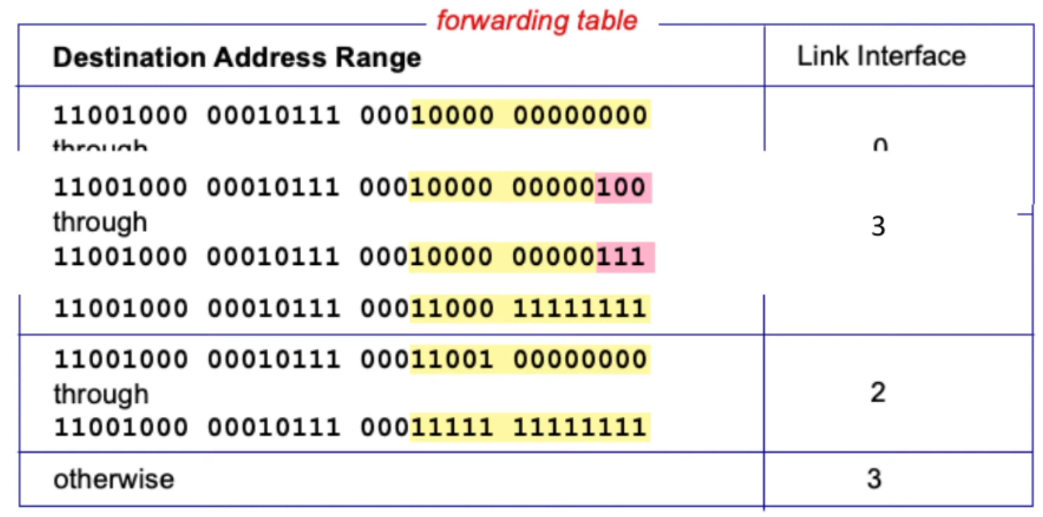
\includegraphics[width=0.65\textwidth]{img/cap-04/tabela-de-encaminhamento.png}
                \end{center}

                \item \textbf{Casamento de maior prefixo:} busca o endereço que melhor coincide com o endereço de destino do pacote na tabela.
            
                \begin{table}[h!]
                    \centering
                    \renewcommand{\arraystretch}{1.2}
                    \setlength{\tabcolsep}{6pt}
                    \arrayrulecolor{blue}

                    \begin{tabular}{|l|c|}
                        \hline
                        \textbf{Destination Address Range} & \textbf{Link Interface} \\ \hline
                        11001000 00010111 00010*** ******** & 0 \\ \hline
                        11001000 00010111 00011000 ******** & 1 \\ \hline
                        11001000 00010111 00011*** ******** & 2 \\ \hline
                        \textit{otherwise} & 3 \\ \hline
                    \end{tabular}

                    \caption{Tabela de encaminhamento com faixas de endereços de destino e interfaces de saída.}
                \end{table} 

                \textbf{\textcolor{blue}{Examples:}} \\[2pt]
                \texttt{11001000 00010111 00010110 10100001} \quad \textcolor{blue}{which interface? 1 } \\
                \texttt{11001000 00010111 00011000 10101010} \quad \textcolor{blue}{which interface? 2 }

                \item Geralmente, usa-se alta performance com TCAMs (memória ternária de conteúdo), permitindo o casamento em apenas um ciclo de clock.

            \end{itemize}

        \subsubsection*{Matrizes de Comutação} 

            \begin{itemize}[left=0.5cm, align=left, nosep]
                \item Transportam pacotes da interface de entrada até a interface de saída apropriada
                \item \textbf{Taxa de comutação :} Velocidade com que pacotes podem ser transferidos das entradas para as saídas \\
                    $\hookrightarrow$ Frequentemente medida como múltiplo da taxa de linha de entrada/saída; \\
                    $\hookrightarrow$ Taxa ideal = $N \times R$ (onde $N$ = número de entradas e $R$ = taxa dos enlaces das interfaces).
                    
                \begin{center}
                    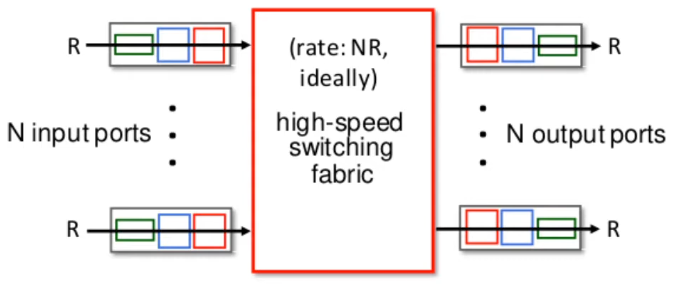
\includegraphics[width=0.65\textwidth]{img/cap-04/taxa-de-comutacao.png}
                \end{center}

                \item \textbf{Formas de implementação :}
                \begin{center}
                    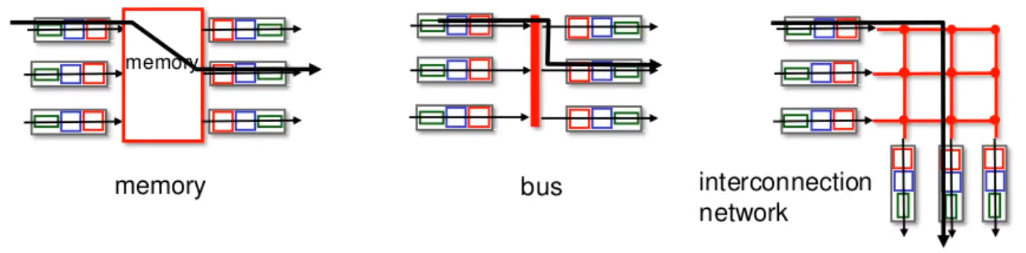
\includegraphics[width=0.65\textwidth]{img/cap-04/implementacao-matriz-de-comutacao.png}
                \end{center}

                \item \textbf{Memória :} \\ 
                    $\hookrightarrow$ Roteadores da primeira geração \\
                    $\hookrightarrow$ Usam computador tradicional com duas placas de rede \\
                    $\hookrightarrow$ Pacote é copiado para a memória do sistema antes do encaminhamento \\
                    $\hookrightarrow$ Problemas :
                    \begin{itemize} 
                        \item Contenção de barramento (depois que utilizado um barramento ninguem pode mais utiliza-lo)
                        \item Passagem dupla do pacote pelo barramento, limitando a velocidade.
                    \end{itemize}
            
                \begin{center}
                    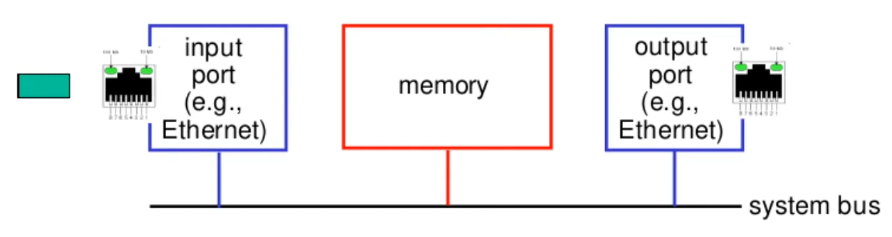
\includegraphics[width=0.65\textwidth]{img/cap-04/matriz-de-comutacao-memoria.png}
                \end{center}

                \item \textbf{Barramento :} \\
                    $\hookrightarrow$ Datagrama sai da porta de entrada para a porta de saída por um barramento compartilhado \\
                    $\hookrightarrow$ Contenção do Barramento : Limitação de velocidade pela banda do barramento. \\
                    $\hookrightarrow$ Restrição de contenção do barramento, uma vez que tem um pacote trafegando no barramento ninguem pode mais trafegar 
            
                    \begin{center}
                        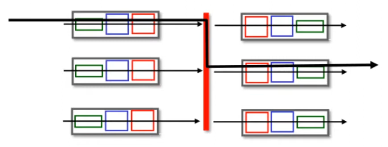
\includegraphics[width=0.65\textwidth]{img/cap-04/matriz-de-comutacao-barramento.png}
                    \end{center}

                \item \textbf{Interconexão :} \\
                    $\hookrightarrow$ Barra cruzada: série de barramentos interconectados, permitindo algum nível de paralelismo; \\
                    $\hookrightarrow$ Continua ocorrendo contenção
                    
                    \begin{center}
                        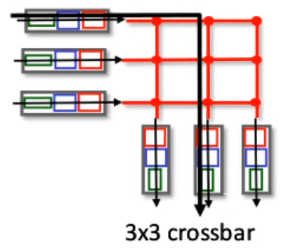
\includegraphics[width=0.55\textwidth]{img/cap-04/barra-cruzada.png}
                    \end{center}

                \item Comutação em múltiplos estágios: consiste em switches \(n \times n\) compostos por vários estágios, estruturados como uma interconexão de matrizes de comutação menores. \\
                    $\hookrightarrow$ Permite níveis de paralelismo. \\
                    $\hookrightarrow$ Fragmenta o datagrama em células de tamanho fixo, possibilitando a paralelização do envio dessas células. \\
                    $\hookrightarrow$ Comuta as células através da matriz de comutação e remonta os datagramas na saída.
                
                    \begin{center}
                        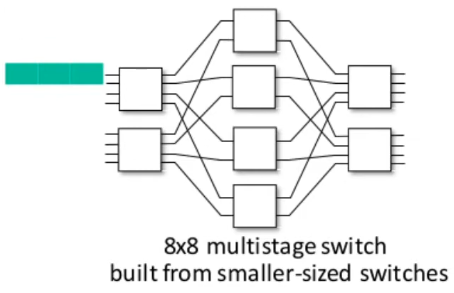
\includegraphics[width=0.65\textwidth]{img/cap-04/comutacao-em-multiplos-estagios.png}
                    \end{center}

                \item É possível escalar esse processo ainda mais parelizando as matrizes de comuração
                
                    \begin{center}
                        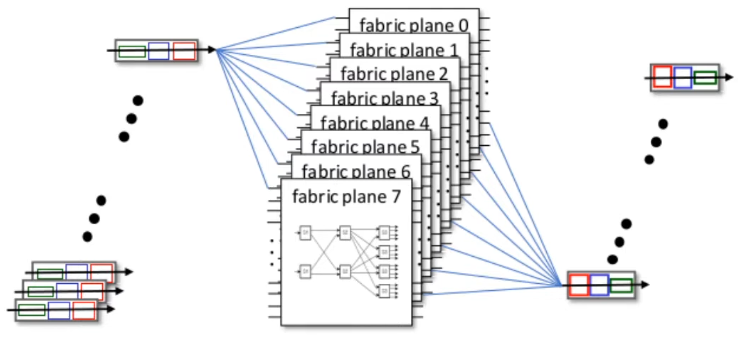
\includegraphics[width=0.65\textwidth]{img/cap-04/multiplos-estagios-escalavel.png}
                    \end{center}
            
            \end{itemize}

        \subsubsection*{Enfileiramento em Interfaces}    

            \begin{itemize}[left=0.5cm, align=left, nosep]
                \item Enfileramento na interface de entrada \\
                    $\hookrightarrow$ Se a matriz de comutação é mais lenta do que as portas de entrada combinadas $\rightarrow$ enfileramento ocorrerá na entrada de filas. \\
                    $\hookrightarrow$ Head of Lines (HOL) blocking : um datagrama enfileirado na frente da fila previne outros na fila de moverem para frente.     

                    \begin{center}
                        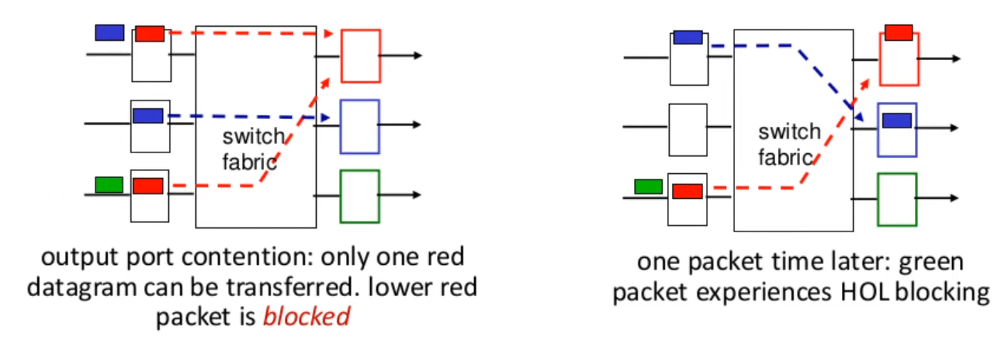
\includegraphics[width=0.65\textwidth]{img/cap-04/hol.png}
                    \end{center}

                \item Enfileramento na interface de saida \\
                    $\hookrightarrow$ Buffering (Descarte): É necessario quando datagramas chegam da matriz de comutação mais rápidos do que a taxa de transmissao do enlace \\
                    $\hookrightarrow$ Politica de descarte ? 
                        \begin{itemize}[left=0.5cm, align=left, nosep]
                            \item Datagramas podem ser perdidos devido ao congestionamento,falta de buffer
                        \end{itemize}
                    $\hookrightarrow$ Disciplinas de escalonamento : formas de lidar com a organização dos pacotes nessa fila de interface de saida para permitir priorizar trafego ou eventualmente reduzir o impacto do infileiramento na comunicação fim a fim     
                       
                    \begin{center}
                        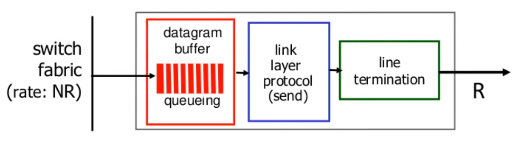
\includegraphics[width=0.65\textwidth]{img/cap-04/enfileiramento-interface-saida.png}
                    \end{center}

                    \begin{center}
                        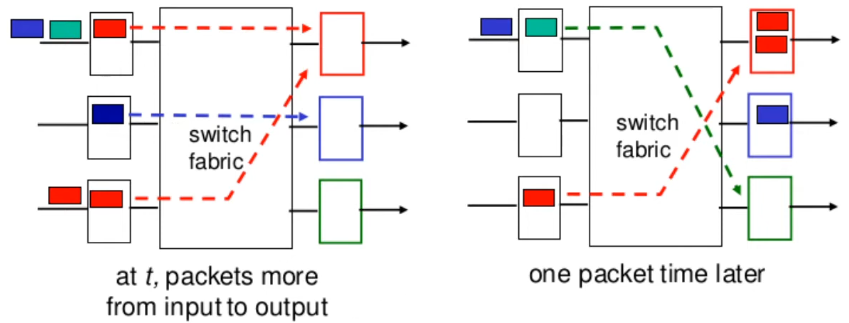
\includegraphics[width=0.65\textwidth]{img/cap-04/enfileiramento-interface-saida2.png}
                    \end{center}

                    $\hookrightarrow$ Descarte quando a taxa de chegada via switch excede a velocidade de linha de saida \\
                    $\hookrightarrow$ Enfileiramento (atraso) e a perda devida o overflow(transbordo) do buffer da porta de saida

                    $\hookrightarrow$ \textbf{Quanto de memoria é preciso se alocada para essa fila ?}
                        \begin{itemize}[left=0.5cm, align=left, nosep]
                            \item RFC 3429 : quantidade de buffer necessario para alocar será RTT vezes a capacidade do enlace C.
                            \item Recomendações recentes : com $n$ fluxos, $buffering = RTT * C / \sqrt{N}$
                            \item Porém muito buffer pode causar atraso (praticularmente em roteadores domesticos)
                            \begin{itemize}[left=0.5cm, align=left, nosep]
                                \item RTTs longos : desempenho ruim para aplicações de tempo real,
                                \item recordar que o atraso baseado no controle de congestionamento  
                            \end{itemize}
                        \end{itemize}
    
                \item Manejamento do Buffer (AQM) \\
                     $\hookrightarrow$ Gerenciar o uso das filas \\
                     $\hookrightarrow$ Descarte : qual pacote adicionar, e qual descarta quando o buffer está cheio 
                        \begin{itemize}[left=0.5cm, align=left, nosep]
                            \item Descarta da cauda : descarta pacote chegando
                            \item Prioridade : descartar/remover baseado em uma prioridade 
                        \end{itemize}    
                    
                    $\hookrightarrow$ Marcação : qual pacotes marcar para sinalixar um congestionamento (ECN,RED)

                    \begin{center}
                        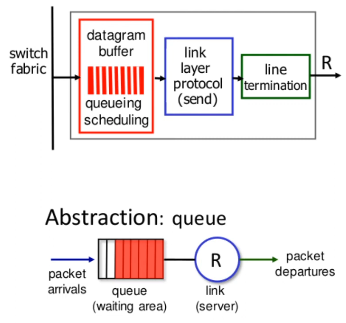
\includegraphics[width=0.35\textwidth]{img/cap-04/manejamento-buffer.png}
                    \end{center}
               
            \end{itemize}
            
        \subsubsection*{Pacotes de Escalonamento :}
            \begin{itemize}[left=0.5cm, align=left, nosep]
                \item Decidir qual o proximo pacote que sera transmitido no enlace
                
                \item \textbf{FCFS} (Firt Come,FIrst Server): Pacotes são transmitidos em ordem atraves da porta de saida \\
                    $\hookrightarrow$ FIFO

                \item \textbf{Prioridade} : \\
                    $\hookrightarrow$ Classifica os pacotes chegados enfileirado-os em classes de acordo com a prioridade.
                        \begin{itemize}[left=0.5cm, align=left, nosep]
                            \item Qualquer campo do cabeçalho pode ser usado para a classificação
                        \end{itemize}    
                    $\hookrightarrow$ Envia pacotes com maiores prioridade na fila que tem pacotes bufferizados     
                        \begin{itemize}[left=0.5cm, align=left, nosep]
                            \item FCFS sem a classe de prioridade
                        \end{itemize}  

                    \begin{center}
                        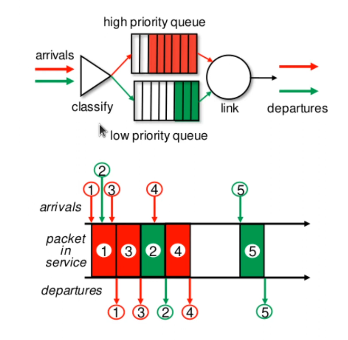
\includegraphics[width=0.45\textwidth]{img/cap-04/prioridade.png}
                    \end{center}
               
                \item \textbf{Round Robin} : \\
                    $\hookrightarrow$ Classifica os pacotes chegados enfileirado-os em classes de acordo com a prioridade. 
                        \begin{itemize}[left=0.5cm, align=left, nosep]
                            \item Qualquer campo do cabeçalho pode ser usado para a classificação
                        \end{itemize}      
                    $\hookrightarrow$ Servidor ciclicamente,repetidamente escaneia as classes de filas, enviando um pacote completo de cada cada classe(se necessário) a cada turno. 
                    
                    \begin{center}
                        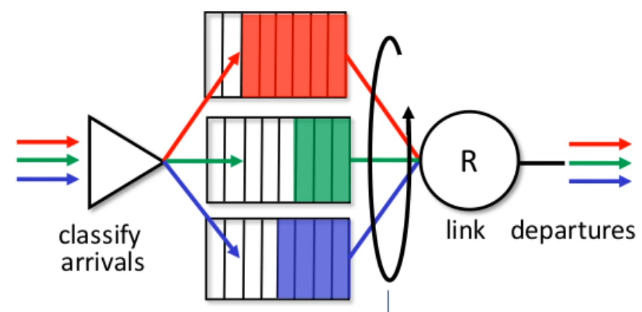
\includegraphics[width=0.65\textwidth]{img/cap-04/round-robin.png}
                    \end{center}
                    
                \item \textbf{Weighted Fair Queues} (WFQ) : \\
                    $\hookrightarrow$ Generalização para o round robin \\
                    $\hookrightarrow$ Cada classe,$i$, tem um peso, $W_i$, e recebe uma quantidade ponderada de serviço em cada ciclo
                        \[
                            \frac{w_i}{\sum_{j}^{} w_j}  
                        \]    
                    
                    $\hookrightarrow$ Banda minima garantida para as classes de baixa prioridade 
                    
                    \begin{center}
                        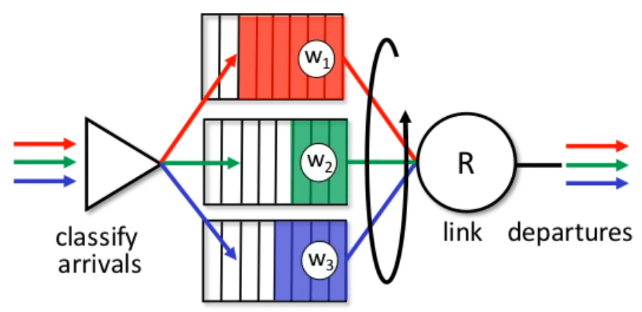
\includegraphics[width=0.65\textwidth]{img/cap-04/wfq.png}
                    \end{center}
            
            \end{itemize} 

    \subsection{IP: Internet Protocol}
    
    \subsection{MiddleBox}

